
\chapter{Problem definition}
\label{cha:problemDef}

In this section we define the problems that have to be solved in order to reach our research goal. Section \ref{sec:mainProblem} presents the high level problem and shows the process we followed in order to identify the features that the system has to provide in order to solve that problem. In Sections \ref{sec:problemDefPlugin} and \ref{sec:problemDefStorage} we identify the sub-problems connected to each of the features. 

\section{High-level Problem}
\label{sec:mainProblem}

As discussed in Section \ref{sec:usemFrm}, the U-Sem paradigm defines how user modelling services are constructed by orchestrating specific types of functional components. It does not, however, provide any formal mechanism or guidelines about how these services and components are constructed and managed in practice. Currently, the only work done in that direction is the adoption of a workflow management system (RDF Gears) which facilitates the orchestration of components into user modelling services. 

Discovering the potential of Social media for user modelling \cite{brusilovsky2007adaptive} has led to an increased demand for U-Sem engineers to design and build many different user modelling services. As a result, engineers are constantly required to implement or adapt variety of functional components that are needed for the new services. Currently, there is a lack of standardized approach and tools that support this process and as a result it requires a lot of manual work and is not efficient. Because of the high demand for user modelling services, the deficiencies in the process have a big negative impact. Our investigation showed that this causes a lot of disturbances and reduced performance to the engineers. Therefore, in this work we investigate whether the current situation can be improved by introducing a user modelling server that is designed to facilitate the process of creating and exposing the user modelling services to the users so that the overhead work of the engineers is limited and they can focus on the core of their work - the user modelling and analysis algorithms.

In order to be able to provide such system we, first, have to identify how engineers work and what are the tasks that require them to do a lot of overhead work and can be potentially fully or partially automated. This is covered in next section.

\section{Overhead tasks}

The task of identifying these overhead tasks is a form of requirements gathering \cite{hickey2004unified} and thus, we investigated the literature to find a suitable approach for doing it. There is a wide variety of possible approaches for requirements gathering \cite{hickey2004unified} : interviews, questionnaires, user observation, workshops, brain storming, role playing, etc. We decided to use the semi-structured interviews technique since it is widely used and it has proved to be effective through the years \cite{dieste2008understanding}.

In order to perform the interviews we first have to identify the stakeholders. Stakeholders are the people that have some kind of interest in the project. They are the ones that will be affected by the project and thus they are the source for identifying the characteristics of the system we have to build. In our case the main stakeholders are the engineers that are already using or will use the U-Sem approach for constructing user modelling services. 

Having identified the target people we performed the interviews, the results of which are summarized in the next section. 

\subsection{Identified overhead tasks}
\label{sec:features}

We carefully analysed all the raw information that was gathered from the interviews and we identified several tasks that require engineers to do a lot of overhead work. We presented them to the stakeholders and after some discussions we ended up with the following final list: 

\begin{itemize}

\item \textbf{Access to social media}
Engineers base a lot of their analysis on the information provided by users in the social media. However, each social media web site provides access through a special API. Currently, each engineer has to implement a component for retrieving the required data from each type of social media he uses. Engineers report that this require them to invest considerable time and efforts.

\item \textbf{Plug in functional components}
The nature of engineers' work is very dynamic. They are constantly required to build new and improve and adapt existing user modelling services. In order to do that they usually have to create and plug into the system new RDF Gears functions and other functional components. Currently this process is done manually and represents major overhead for the engineers.

\item \textbf{Data management} 
Many of the engineers build services that need to store various types of data(e.g. intermediate and final results). Currently, they are forced to manually set-up databases and program the components needed for interacting with each type of data. This is usually not a trivial task, it requires time and knowledge and therefore, it resembles a big overhead to the engineers.

 
\item \textbf{Integration with Hadoop}
The amount of information that has to be processed in the system can sometimes be huge. Therefore, sometimes, it has to be processed by external Hadoop based systems. Currently, engineers have to manually manage the exchange the information to and from the Hadoop systems.

\item \textbf{Scheduled execution of services}
Some services require to be executed on regular bases. For example, a service that has to monitor how certain user profile changes over time might need to be executed daily. Currently, this execution has to be manually accommodated by the engineers and it becomes a serious overhead when they are responsible for many services like that. 

\end{itemize}

Having identified the tasks that engineers find most problematic allows us to rephrase our goal into providing a solution that is designed to facilitate these tasks. Facilitating each of these tasks is a feature that the system has to provide. The limited scope of this thesis work, however, does not allow us to cover all of the these features and therefore, we are focusing only on providing the features that will bring the most advantage for the engineers. In order to do that, we have to prioritize them based on the impact they will provide. 

\subsection{Features prioritization}

Prioritizing the features is not a trivial task because each of the stakeholders has a slightly different view on the benefits provided by each of the features that we already identified. Therefore, we performed a research in order to find a suitable approach for dealing with this situation.

Requirements prioritization is a relatively old research topic and there are numerous approaches that are currently available \cite{moisiadis2002fundamentals}. The most popular include Quality Function Deployment (QFD) \cite{chan2002quality}, the Analytical Hierarchy Process(AHP) \cite{roper1990analytic} , as well as a variety of industrial practices such as team voting \cite{moisiadis2002fundamentals}, etc. However, literature also suggests that there is no perfect solution for this problem and the applicability of each approach depends greatly on the particular situation it is used in.

For our project, we choose the analytic hierarchy process approach \cite{roper1990analytic}. This decision was based on the fact that it is especially suitable for prioritizing a small number of requirements\cite{karlsson1997cost} and it is a proven and widely used \cite{karlsson1998evaluation}. In literature, as a disadvantage of this approach is considered the fact that it takes no account of interdependencies between requirements \cite{roper1990analytic}. However, this issue is not a problem for our solution because the project's high-level features that we want to prioritize are loosely coupled and they have little dependency between each other. 


\subsubsection{Features prioritization using AHP}
In the Section \ref{sec:features} we identified five high-level requirements(features) that cover the main functionality of the system. In this step we are using the AHP's pairwise comparison method in order to assess the relative value of each of them. It basically requires the stakeholders to systematically evaluate the importance of each of the features by comparing them to one another two at a time. Then, the AHP converts these evaluations to numerical values which represent the priority of each of the features. In order to perform this process, we instructed the stakeholders on the process and asked them to perform the evaluations by filling in a specially prepared form which is presented in Appendix \ref{cha:priority}.

We let the participants to work alone, defining their own pace. We also allowed them to choose the order of the pair's comparison. Discussions were also allowed. When all participant finished the pairwise comparison, as advised in \cite{karlsson1997cost} we had to make sure that the provided results are consistent. In order to do that we had to calculate the the consistency indices of the pairwise comparisons. According to \cite{karlsson1997cost} values lower than 0.10 are considered acceptable and even values around .12 are commonly achieved in the industry and can also be considered acceptable. The calculation showed that two of the participants have indices higher than .23 which indicates serious inconsistencies (table \ref{tbl:reqInitialConsist}). Therefore, we asked them to revise their answers and the results afterwards measured values that are acceptable (table \ref{tbl:reqFinalConsist}).
 
 \begin{table}[h!]
  \begin{center}
    \begin{tabular}{| l | l | l | l | l |}
    \hline
    & Stakeholder 1 & Stakeholder 2 & Stakeholder 3 & Stakeholder 4 \\	 \hline
    Consistency ratio & 0.04 & 0.23 & 0.13 & 0.26 \\
    \hline
    \end{tabular}
  \end{center}
  \caption{The initial consistency ratios for each of the stakeholders.}
  \label{tbl:reqInitialConsist}
\end{table}


 \begin{table}[h!]
  \begin{center}
    \begin{tabular}{| l | l | l | l | l |}
    \hline
    & Stakeholder 1 & Stakeholder 2 & Stakeholder 3 & Stakeholder 4 \\	 \hline
    Consistency ratio & 0.04 & 0.12 & 0.13 & 0.11 \\
    \hline
    \end{tabular}
  \end{center}
  \caption{Consistency ratios for each of the stakeholders after refinement.}
  \label{tbl:reqFinalConsist}
\end{table}

Once we had achieved satisfying results we calculated the distributions and outlined the candidate requirements in a diagram (Figure \ref{fig:reqPriority}). Each requirement's determined value is relative and based on a ratio scale. Therefore, a requirement whose value is calculated as 0.20 is twice as valuable as a requirement with a value of 0.10. Additionally, the sum of the values for all requirements equals 1. This means that a requirement with a value of 0.10 provides 10 percent of the value of all the requirements.

\begin{figure}[h!]
  \centering
      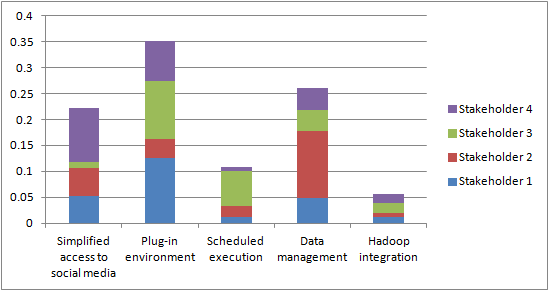
\includegraphics{requirements/value_diagram.png}
  \caption{The value distribution of the 5 requirements in the U-Sem project.}
  \label{fig:reqPriority}
\end{figure}


Finally, based on the provided results from the prioritization and because of the limited scope of this thesis we decided to design and implement the two features that will provide the most benefits for the users: "Plug-in Environment" and "Data Management". Next sections cover in details the problems connected to each of the two features.

\section{Plug-in Environment}
\label{sec:problemDefPlugin}

During the initial interviews with the engineers that are going to potentially use the system, we uncovered that the nature of their job is very dynamic. In their day to day work they are expected to constantly improve and come up with new user modelling services. As a result, they are continuously producing new software code that implements the new functional components that are needed for building the services. After each production cycle, the program code has to be deployed into U-Sem so that it is available for testing, demonstration and evaluation purposes. Currently, this process is mostly done manually by engineers who claim that it takes them a lot of time, efforts and is a source of problems that are hard to find. Therefore, the problem that we have to solve is to design a solution that facilitates this process. 

In order to be able to fully understand the problem we, first, have to fully understand how this process is currently performed. Therefore, we performed additional interviews with the engineers which showed that currently engineers follow the following process: First, they check out the latest source code of the wokrflow engine (RDF Gears) system from the source code repository and import it in their Eclipse IDE. Then, they extend it by adding the source code and other resources required for the new functional components that they build. Afterwords, they have to build and deploy the system to a web server to make it available for testing. If not satisfied with the end result, engineers apply the necessary changes and follow the build, deployment and test steps again. At the end, they have to commit the new version of the system back to the source code repository.

Analysing this process we concluded that it is far from optimal, it is error prone and it can bring a lot of discomfort to the engineers working with the system. The reasons behind this statement and also the sub-problems that have to be solved by the solution are the following:

\begin{itemize}

	\item The process requires a lot of time and efforts from the engineers engineers because it involves many tasks that are considered as overhead by engineers since they are not part of the core of their work and have to be repeated every time a functional component is added to the system.
	
	\item The deployment step of the process requires engineers to restart the web server where the system is deployed. As a result, during the time the server is down all other running services are unavailable. This is a major problem for everyone that is using the system during that time.
	
	\item Another serious problem comes from the fact that every step of the process requires engineers to have certain kind of knowledge in order to be able to perform it. As a result, the training period for new engineers is significantly increased. This may easily cause project delays and missed deadlines.
	
	\item Multiple engineers performing the process simultaneously may result in loss of functionality. Figure \ref{fig_vers_prob} illustrates the problematic scenario. As stated earlier, in order to add new functionality, engineers must first check out the source code of the system, make the changes and deploy the new version on the web server. However, if two engineer perform this process simultaneously then the new functionality provided by the first engineer will be lost when the second one deploys his version. 
	
	\begin{figure}[h!]
  \centering
  	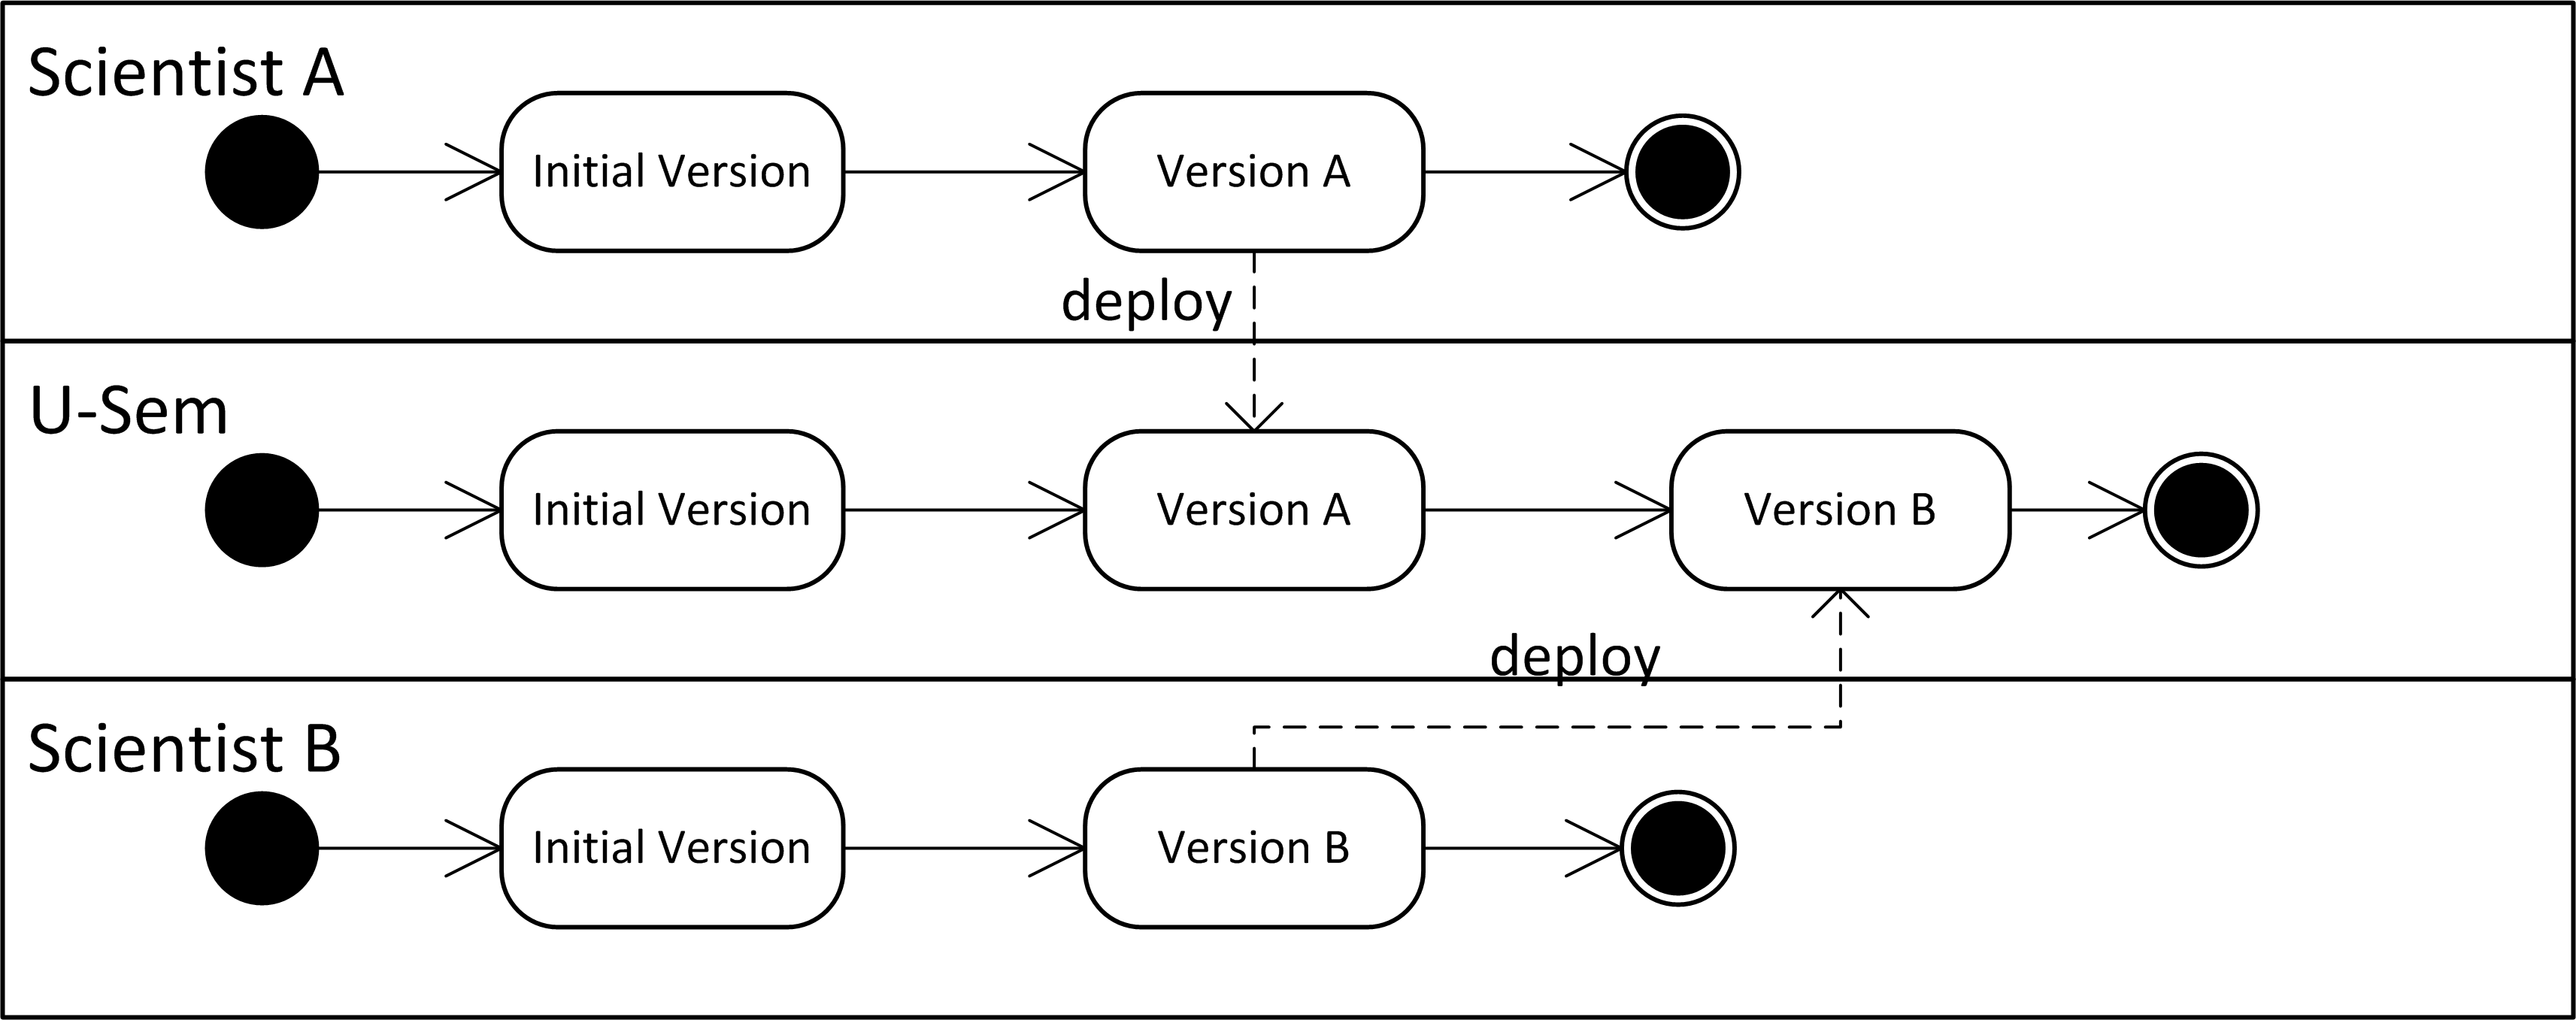
\includegraphics[scale=0.75]{plug-in/version_problem.png}
  \caption{State diagram illustrating the scenario where two engineers extend U-Sem simultaneously and the changes made by engineer A are lost.  }
  \label{fig_vers_prob}
\end{figure}
	
	\item Engineers also reported that following the current process the source code implementing the different functional components resides in the same project and as a result, they have become, over time, tightly coupled between each other. This has made them very hard to be maintained and extended.
		
\end{itemize}

We believe that providing a solution that overcomes these problems will significantly improve the current situation enabling engineers to focus more on the core of their work. In next section, we cover the "Data Management" issue and identify the problems hiding behind it.


\section{Data Management}
\label{sec:problemDefStorage}

The interviews that we performed with the engineers showed that many of the services they implement require functional components that provide means for executing data storage and retrieval operations. They reported that the structure and semantics of the data and the particular operations they have to perform on it varies a lot but the main scenarios can be classified in the following groups:

\begin{itemize}

	\item \textit{Raw data} - Engineers reported that most of the modelling services they build are based on the social media. Basically, they have to retrieve certain entries (e.g tweets from Twitter ) which are the basis for the user modelling. In certain cases engineers have to store this "raw data" locally. Usually, this is as a result of the fact that retrieving the entities from the social media web sites is time consuming and also some of the APIs limit the number of entities one can get for a certain amount of time \cite{cheong2009integrating}. This makes the execution of workflows slow because the system has to wait to get the needed entries every time. Therefore, engineers are forced to store these entries locally and only make sure they are up-to-date prior to the execution of a workflow.
	
	\item \textit{User provided data} - Some services require information that is not available from social media and has to be provided by the users of the system. For example, in certain use-cases users have to fill in questioners so that the results from future user modelling are adjusted based on the answers provided by the users. It is infeasible to ask the users for that information every time the service is executed and that is why it has to be stored within the system.
	
	\item \textit{Intermediate results} - Some services consist of two phases. The first phase continuously calculates some intermediate representation of the raw data. In the second phase, on user request the final result is calculated based on the intermediate data. One such example is the Twinder service \cite{tao2012twinder}. Therefore, between the two phases, the intermediate results have to be stored and later retrieved back.
	
	\item \textit{User profiles} - Some services require that users are able to monitor how the generated user profiles evolve over time. For example, in e-learning systems users want to be able to see how the knowledge of a certain person has changed after following a certain course in order to measure how helpful the course was for that person. Therefore, every time a service is executed the results have to be stored so that they can be further analysed later.
	
	\item \textit{System data} - Finally, many of the features of the system need to store some kind of information. For example, the user authentication functionality has to store all kind information about the users of the system: user names, passwords, privileges, etc. The scheduling feature has to store information about the time at which each service has to be executed. 
	
\end{itemize}

Clearly, there are a lot of scenarios that require data storage and retrieval operations and currently, the system does not provide any means to support engineers in defining workflows that require such operations. Each engineer is responsible to set up a database server and create custom RDF Gears components that serve the particular needs. However, this process requires a lot of time and efforts, and suffers from many downsides and problems:

\begin{itemize}
	\item \textit{Knowledge required} - designing and implementing components for dealing with persistent data is not a trivial job and requires specific type of knowledge. Many of the engineers building services have mathematical or statistical backgrounds and are likely not to have in depth knowledge in the database field. In order to be able to build their services they have to acquire this knowledge which can cause significant overhead and waste of time. Additionally, the fact that they are not professionals in the field may lead to problems and shortcomings.
	
	\item \textit{Server administration} - Most of the storage solutions require setting up a dedicated database server. These servers have to be hosted somewhere, maintained, backuped, etc. All these tasks require a lot of effort and if every user has to do it, it will result in large amount of duplicated work and overhead. If engineers decide to use a shared database server then appears the question of who is responsible to manage it and ensure its security and privacy.
	
	\item \textit{Dynamic data structure} - It is expected that the structure of the stored data might change over time. When a database with fixed schema is used (like most SQL solutions) then every time the structure changes the engineers have to connect to the database and apply the changes manually. This task is likely to be annoying, time consuming and even error prone for some engineers. Therefore, automating this process can save time to engineers and reduce the number of mistakes caused by carelessness. 
	
	\item \textit{Collaboration} - collaborations between engineers on data level is reported to be quite important and can save them a lot of time. Currently, there are no facilities available to support that requirement. Engineers have to organize this collaborations personally. Additionally, because the collaborations are not integrated in the system they are likely to be hard to monitor and control.
	
	\item \textit{RGL translation} - Generally available database solutions are not capable to deal with data in the RGL format introduced in RDF Gears. Therefore, every single component that deals with persistent data has to translate the RGL values to values compatible with the database solution and vice versa. Clearly, all this code is redundant and removing this responsibility from the engineers will save them time and efforts so that they can focus their attention to the core of their work.
	
	\item \textit{RDF Gears and components with side effects} - Components that store data are components that have side affects. However, as discussed in Section \ref{sec:backRDFGears} RDF Gears is not designed to work with such components and some unexpected behaviour might be expected. Therefore, engineers building components with side effects that are not aware of the way RDF Gears operate internally risk to introduce problems that may be also hard to detect.
	
\end{itemize}

In this thesis we aim to propose a solution that is capable to overcome these problems and save engineers a lot of time, efforts and prevent mistakes while dealing with persistent data.

\section{Conclusion}

In this chapter we identified the problems that we have to overcome in order to achieve our research goal. In order to do that we conducted series of interviews and identified the features that have to be provided by the system. We evaluated the importance of each of the them and chose to focus our work on the two areas which were indicated to be most beneficial for the engineers: "Plug-in environment" and "Data Management". We further investigated both of them in order to identify the sub-problems that have to be solved for each of them. Next chapters are dedicated to each of the two areas and present the architecture and implementation that we propose in order to solve the identified problems. Chapter \ref{cha:plug-in} covers the Plug-in environment and Chapter \ref{cha:data} is dedicated to the Data Management feature.